\documentclass[10pt,twocolumn,letterpaper]{article}

\usepackage{iccv}
\usepackage{times}
\usepackage{epsfig}
\usepackage{graphicx}
\usepackage{amsmath}
\usepackage{amssymb}

% Include other packages here, before hyperref.
\usepackage{algpseudocode}

% If you comment hyperref and then uncomment it, you should delete
% egpaper.aux before re-running latex.  (Or just hit 'q' on the first latex
% run, let it finish, and you should be clear).
\usepackage[pagebackref=true,breaklinks=true,letterpaper=true,colorlinks,bookmarks=false]{hyperref}

 \iccvfinalcopy % *** Uncomment this line for the final submission

\def\iccvPaperID{****} % *** Enter the ICCV Paper ID here
\def\httilde{\mbox{\tt\raisebox{-.5ex}{\symbol{126}}}}

% Pages are numbered in submission mode, and unnumbered in camera-ready
\ificcvfinal\pagestyle{empty}\fi
\begin{document}

%%%%%%%%% TITLE
\title{Randomized Spatio-Temporal Pyramids for Egocentric Activity Recognition}

\author{Tomas McCandless, Kristen Grauman\\
University of Texas at Austin\\
{\tt\small \{tomas, grauman\}@cs.utexas.edu}
% For a paper whose authors are all at the same institution,
% omit the following lines up until the closing ``}''.
% Additional authors and addresses can be added with ``\and'',
% just like the second author.
% To save space, use either the email address or home page, not both
%\and
%Second Author\\
%Institution2\\
%First line of institution2 address\\
%{\tt\small secondauthor@i2.org}
}

\maketitle
%\thispagestyle{empty}

%%%%%%%%% ABSTRACT
\begin{abstract}
	Egocentric video and wearable computing have become increasingly
	prevalent in the past decade, resulting in a huge explosion in the amount
	of video content. In this paper, we develop a novel approach for
	activity recognition using the UC Irvine ADL (Activities of Daily Living)
	dataset \cite{Ramanan12}. The ADL dataset consists of hundreds of egocentric video clips
	for dozens of people performing various everyday activities in their own
	homes, often related to hygeine or food preparation. Frames in the dataset
	are annotated with bounding boxes for detected objects and hand positions, 
	activity labels, and each object is marked as active or passive depending
	on whether it is being interacted with. We partition video clips into
	3-dimensional cuboids, based on many different multi-level partitioning
	schemes,then concatenate object histograms
	over multiple levels to form feature vectors which we use to train a pool
	of weak SVM classifiers. Finally, we use a boosting algorithm to form a
	final strong classifier with performance similar to the current state of
	the art.
\end{abstract}

%%%%%%%%% BODY TEXT
\section{Introduction}
	Activity recognition is becoming an increasingly canonical problem in
	computer vision as researchers are beginning to explore the domain more
	thoroughly and several relevant datasets have been released. The problem 
	of human activity recognition is in some ways less well defined
	than, say, object recognition for 2D images, in part due to the relative
	lack of datasets for activity recognition, and also because it is somewhat
	problematic to define a canonical representation for each type of action.
	In other words, it seems as though there can be higher intra-class
	variation for activity recognition than for, say, object recognition. 
	% past datasets scripted activities
	Datasets geared towards activity recognition in the past have often
	consisted of actors performing scripted activities in a static and at
	times artificial environment, yet in order to develop robust and effective
	methods, we need datasets that are more organic in the sense that they
	depict unscripted activities in a natural environment such as the home of
	a subject \cite{Ramanan12}. 
	% similarity of problems, occlusion, clutter
	However, activity recognition and object recognition do share some
	similar properties. For instance, occlusion and background clutter are
	problems that arise in both problems.

\subsection{Applications}
	% application to life logging
	A recent trend in wearable computing is so-called life logging which can
	assist patients suffering from memory loss \cite{Sellen07}. However, with
	such large amounts of video, it becomes necessary to have a system for
	efficiently browsing video. A robust egocentric activity recognition
	system could automatically tag video clips with types of activities (this
	could be done either online or offline), thus allowing the user to, for
	instance, quickly find all clips in the past that depict making tea.

	% application to senior living
	There are many clinical benchmarks used to evaluate patients everyday
	functional abilities \cite{Kopp97, Catz97, Itzkovich07}. 
	These benchmarks are currently conducted in a
	hospital setting, but a robust system for egocentric activity recognition
	could greatly impact the workflow for patient evaluation, as such a system
	would allow for passive long term observation of patients in their own
	homes. This could lead to more accurate evaluations since it would be
	possible to collect far more data about individual patients. Such a system
	would also eliminate the need for patients to commute to a hospital to have
	evaluations done, thus reducing cognitive and physical burden on patients.
	
	% TODO application to law enforcement

%-------------------------------------------------------------------------
\subsection{Related Work}


	In \cite{Laptev08}, Laptev \etal investigate aligning movie scripts with
	video for the purpose of annotating human actions, and achieve 91.8\%
	accuracy on the KTH dataset.
	
	In \cite{Marszalek09}, Marszalek \etal released a novel dataset based on
	Hollywood movies that contains twelve types of activities and ten
	different classes of scenes. The main contribution of this paper is based
	on the observation that the visual content of a human's environment can
	impose useful constraints on the type of activity occurring. For instance,
	food preparation activities frequently occur in a kitchen environment. In
	particular, Laptev \etal show how to learn relevant scene classes along
	with any correlations they may have with human activity.
	
	In \cite{Fathi12}, Fathi \etal focus on the relationship between gaze and
	activity recognition in an egocentric settting and develop methods to
	predict activity given gaze, gaze given activity, and to predict both
	activity and gaze. The activities in this
	published dataset are primarily related to food preparation. 
	
	The main work related to our own is that carried out in \cite{Ramanan12}. 
	In this work the ADL dataset is introduced as well as detailed analysis of
	performance of several different classifiers. The ADL dataset consists of
	roughly 10 hours of video in total, collected from 20 people performing
	18 types of unscripted actions in their own homes. There are 26 different 
	types of detected objects, including 5 active and 21 passive objects. 
	The crucial contribution of
	\cite{Ramanan12} is that egocentric activity recognition is ``all about
	the objects'', particularly the objects being iteracted with, as
	recognition accuracy increases dramatically when ground truth object
	locations rather than detected locations are used to train the classifier. 

	\begin{figure}[t]
		\begin{center}
			%\fbox{\rule{0pt}{2in} \rule{0.9\linewidth}{0pt}}
			  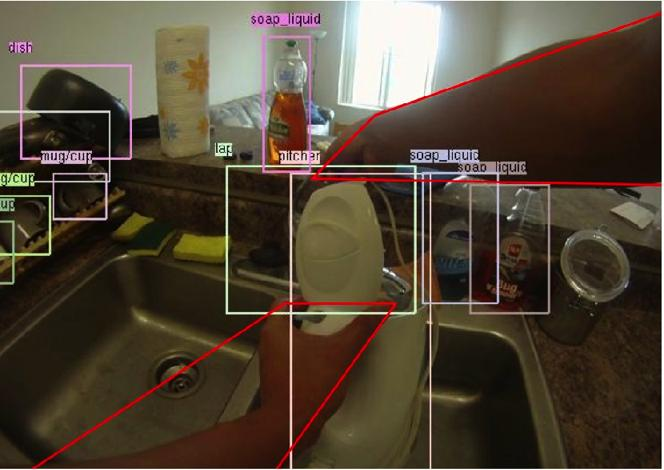
\includegraphics[width=0.8\linewidth]{/u/tomas/thesis/figures/thumbnail.jpg}
		\end{center}
		   \caption{An example frame with annotations TODO: find a better image}
				\label{fig:long}
				\label{fig:onecol}
	\end{figure}
	
	Our algorithm is inspired by the work of \cite{Jiang12}, which uses a
	similar boosting approach with randomized spatial pyramids for 2D images, 
	leading to increased robustness to intra-class variation. The proposed
	method is benchmarked on three public datasets.

	% yong jae segmentation
	% work from other researchers on segmentation
	% work from other researchers on activity recognition with other modes of
	% sensor data

\section{Approach}
	Our algorithm was inspired by the work of \cite{Jiang12}. We use a
	version of the SAMME Ada-boost algorithm \cite{Zhu06}, as follows:

	\textbf{Algorithm 1} Training RSTP Classifier via Boosting \\
	\textbf{INPUT:} 
	\begin{itemize}
		\item $N$ labeled training videos $\Phi = \{(V_i, c_i)\}_{i=1}^N$
		\item A pool of partition patterns $\Theta = \{\theta\}$
	\end{itemize}
	\textbf{OUTPUT:}
	\begin{itemize}
		\item A strong video classifier $F$. For an unlabeled video $V$, 
			$c=F(V)$ is the predicted label for $V$.
			\begin{enumerate}

				\item For each $\theta \in \Theta$
					\begin{itemize}
						\item Train a multi-class classifier (SVM) $f_\theta$ on $\Phi$
					\end{itemize}

				\item Initialize:
					\begin{itemize}
						\item weight $w_i = \frac{1}{C N_{c_i}}$ for each video clip,
							where $N_{c_i}$ is the number of videos with label $c_i$.
						\item current iteration number $j=0$.
						\item current accuracy $\sigma_j = 0$.
					\end{itemize}

				\item For each round of boosting:
					\begin{itemize}
						\item increment $j$.
						\item Re-normalize the weight vector: $w_i = \frac{w_i}{\Sigma_i^N w_i}$.
					  \item For each pattern $\theta$, compute its classification
							error $err_\theta$ as the dot product product of $w$ with the indicator
							vector of incorrect classifications using $f_\theta$. 
						\item Choose the pattern $\theta_j$ with minimum error $err_j$
						\item Compute the weight for $\theta_j$ as: \\
							$\alpha_j = \mbox{log} \frac{1 - err_j}{err_j} + \mbox{log}(C
							- 1)$
						\item Update the weight vector:\\
							$\mbox w_i = w_i * \mbox{exp}(\alpha_j *
							\mbox{\textbf{I}}(f_{\theta_j}(V_i) \neq c_i))$.
						\item Generate the strong classifier: \\
							$F(V) = \mbox{arg max}_c \Sigma_{m=1}^j \alpha_m *
							\mbox{\textbf{I}}(f_{\theta_m}(V) = c)$
					\end{itemize}

			\end{enumerate}
	\end{itemize}

\subsection{Biased Partitions}
	Initially, all randomized partitions were computed according to a uniform
	distribution. However, in an attempt to avoid generating partition schemes
	that are not sufficiently discriminative, we bias the partition generation
	step according to computed distributions of active object locations across
	training data. 

	\begin{figure}[t]
		\begin{center}
			%\fbox{\rule{0pt}{2in} \rule{0.9\linewidth}{0pt}}
			  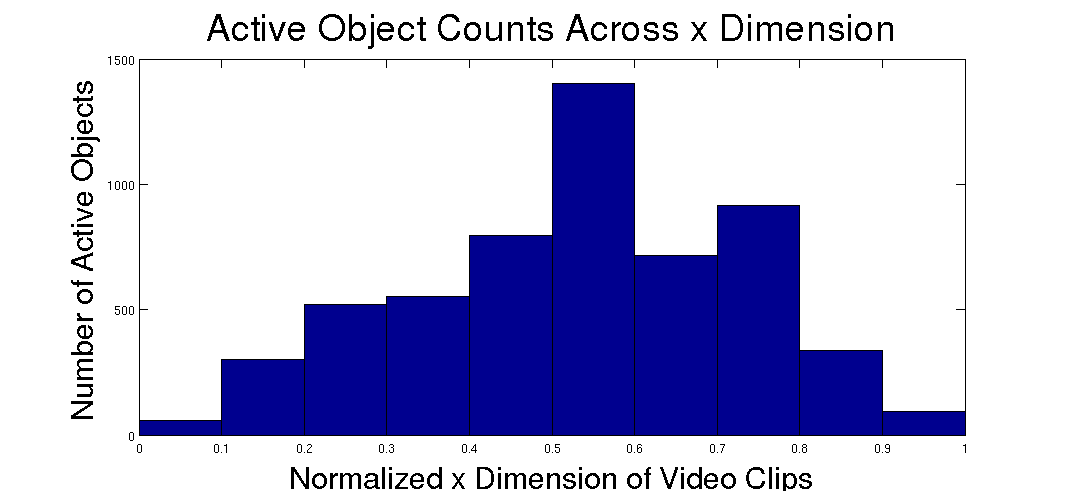
\includegraphics[width=1.0\linewidth]{/u/tomas/thesis/figures/active_obj_distr_x.png}
			  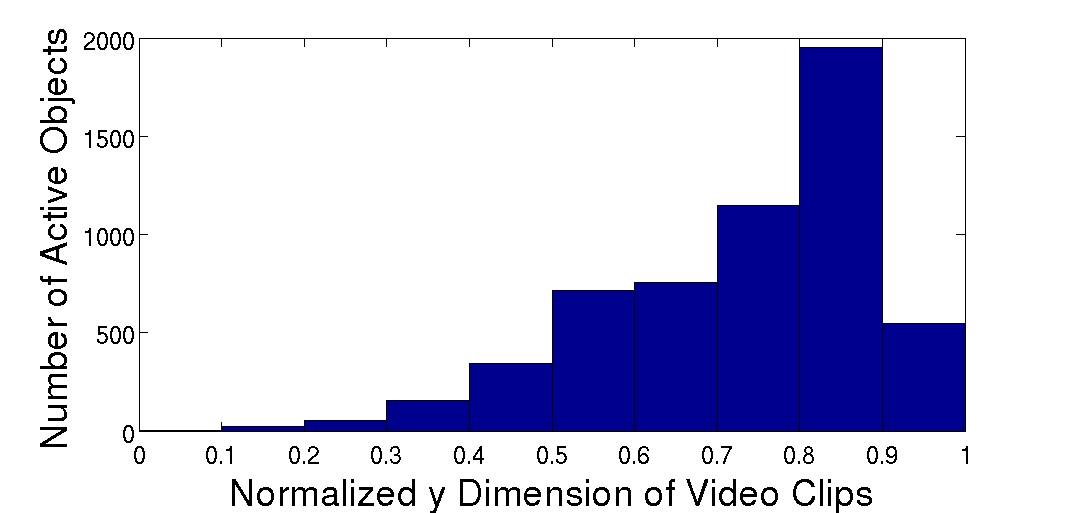
\includegraphics[width=1.0\linewidth]{/u/tomas/thesis/figures/active_obj_distr_y.png}
			  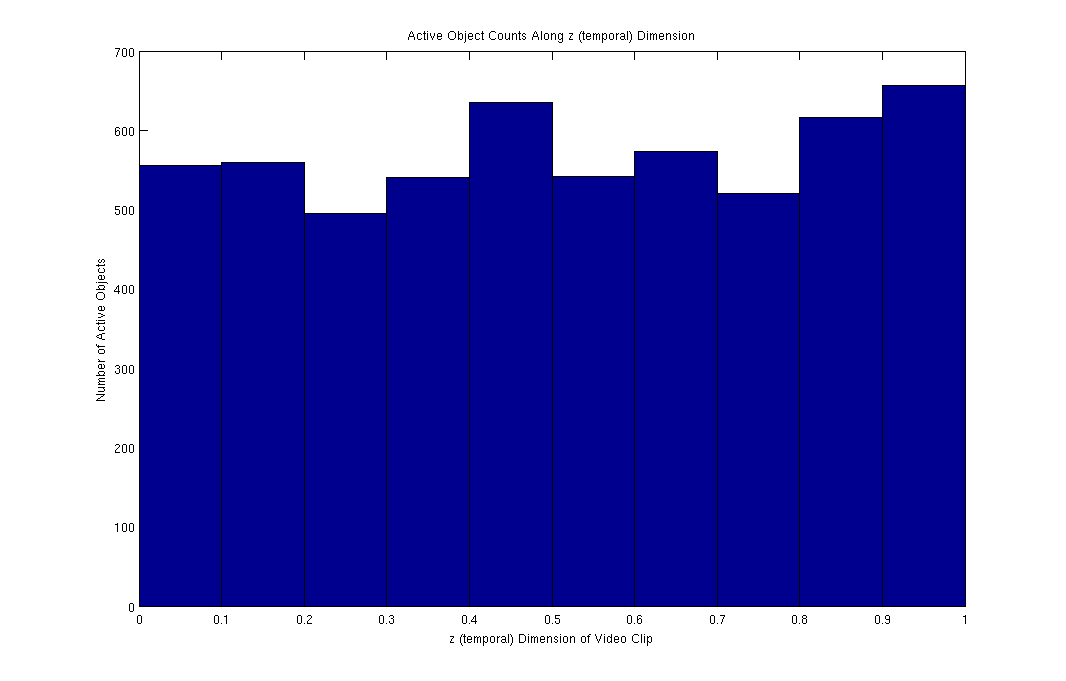
\includegraphics[width=1.0\linewidth]{/u/tomas/thesis/figures/active_obj_distr_z.png}
		\end{center}
		   \caption{Counts of active objects across all 3 dimensions}
				\label{fig:long}
				\label{fig:onecol}
	\end{figure}
	
	From figure 2 we see that active objects tend to occur in the lower center
	of the field of view, and that active objects are nearly uniformly
	distributed across the temporal dimension. This is as expected, because
	the active objects are close to the hands which are in the lower field of
	view from an egocentric perspective. When generating a biased
	partition, we can choose to prefer cutting around regions that tend to
	contain active objects (denoted as bias type 2), or we can choose to prefer 
	cutting through regions that tend to contain active objects (denoted as bias type 3). 
	We denote by bias type 1 the method of using completely uniform
	distributions to generate partitions.
\section{Results}
	The ADL dataset has been modified since the publication of
	\cite{Ramanan12}; because of this, running the published code gives
	slightly lower accuracy than the originally published numbers.

	
	\begin{table}
		\begin{center}
			\begin{tabular}{|l|c|c|c|c|}
				\hline
				Object Type & bag & pyramid  \\
				\hline\hline
				O (published number) & 24.7 & 32.7 \\
			 AO (published number) & 36.0 & 40.6 \\
				\hline\hline
				O (after modification) & 26.6 & 29.0 \\
 				AO (after modification) & 34.9 & 36.9 \\
				\hline
			\end{tabular}
		\end{center}
		\caption{Overall classification accuracy on pre-segmented video clips before and after dataset
		modification}
	\end{table}
	
	The results shown in Table 1 are computed using a form of cross
	validation (use the video clips from person $i$ as a validation set, and
	train on the video clips from the remaining people).
	
\section{Conclusion and Future Work}
	We have presented a novel application of the well-known boosting framework
	with results comparable to the current state of the art. 
	Future work could incorporate different types of biases when generating
	partitions. The ADL dataset also includes annotations for hand positions,
	which we have incorporated implicitly through our generation of partitions
	biased relative to regions which tend to contain active objects. However,
	it could be possible to incorporate explicit information given by hand
	positions to obtain better classification results.
	Additionally, it may be worthwhile to investigate the performance of other
	variants of the boosting algorithm.
% other boosting algorithms

{\small
\bibliographystyle{ieee}
\bibliography{egbib}
}

\end{document}
